\section{Identiteit}

\textit{In dit hoofdstuk wordt de vraag ``Hoe wordt er omgegaan met de identiteit van de gebruiker binnen de implementatie?'' behandeld. Het doel van de vraag is om de mogelijkheden en toepassingen van identiteit te beschrijven aan de hand van de geselecteerde implementaties.}

\begin{figure}[h]
  \centering
  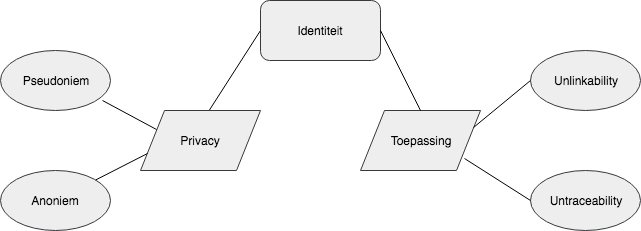
\includegraphics[width=0.8\textwidth]{figures/uitwerking_identity}
  \caption[Opbouw beantwoording ``Identiteit'']{Termen die als leidraad gebruikt zijn om het resultaat te beschrijven}
  \label{opbouw:identiteit}
\end{figure}

\subsection{Aanpak}

In fig. \ref{opbouw:identiteit} is te zien welke componenten er gebruikt zijn om de benodigde informatie te vinden. In het vooronderzoek is er gevonden dat identiteit eigenlijk uit twee onderdelen bestaat binnen Blockchain implementaties. Het privacy gedeelte, wat bepaalt of de identiteit zoals in gebruik bij de implementatie pseudoniem of anoniem is. Daarnaast is de toepassing van de identiteit van belang. Een voorbeeld van de toepassing van de identiteit is bijvoorbeeld het ondertekenen van transacties. 

\subsubsection{Identiteit}

In het vooronderzoek is er ook vastgesteld dat de identiteit van een gebruiker en hoe het gebruikt wordt is terug te leiden naar de architectuur van de Blockchain. De kern van Blockchain implementaties met betrekking tot identiteit en de toepassing daarvan is het gebruik van public- en private key cryptografie. Bij dit onderdeel was het belangrijk om niet teveel te beschrijven van de onderliggende cryptografie, omdat dit buiten de scope van de vraag valt. 

\newpage
\subsection{Conclusie}

\paragraph{Bitcoin} is een public Blockchain waarbij de gehele historie van transacties publiekelijk in te zien is. Een deelnemer in het Bitcoin netwerk wordt geïdentificeerd aan de hand van zijn public key. Deze public key wordt onder andere opgenomen in transacties om de betaler en de ontvanger te registreren. In een studie gedaan door \cite{reid2013analysis} wordt er een analyse model opgezet dat aantoont dat het Bitcoin protocol niet aan de untraceability eis voldoet.

\paragraph{Cardano} is een public Blockchain waarbij de gehele historie van transacties publiekelijk in te zien is. Cardano maakt gebruik van public- en private key cryptografie om pseudonimiteit te waarborgen. Deze keys worden gebruikt om een transactie van een bestemming te voorzien, waarbij er drie definities van adressen gebruikt worden: een public key address, een script address en een redeem address.

\paragraph{EOS} is een consortium Blockchain waarbij gebruikers zichzelf identificeren met een unieke naam van maximaal twaalf karakters. Om te participeren binnen het netwerk dient er toegang verleent te worden door een authenticatie proces alvorens de deelnemer wordt toegelaten.  Handeling binnen het netwerk worden gevalideerd door een Role Based Permissie systeem, waarbij permissies gekoppeld zijn aan actions die vastgelegd zijn in de lokale database.

\paragraph{Monero} is een public Blockchain waarbij de gehele historie van transacties publiekelijk in te zien is. Binnen Monero heeft elke deelnemer een account die gebaseerd is op twee keys: Spend Key en een View Key. Door het afleiden van een eenmalige public key, ook wel een Stealth Address genoemd, uit de Spend Key en View Key garandeert het Monero protocol unlinkability. Untraceability wordt behaald door het gebruik van Ring Signatures. Hierbij worden meerdere Stealth Addresses toegevoegd aan een transactie, waarbij een afkomstig van de verstuurder van de transactie en de rest aangevuld door eerder gebruikte Stealth Addresses in de Blockchain. Hierdoor wordt de herkomst van een transactie gemaskeerd. 